\Chapter{Grafikus szerkesztőeszköz}

\section{A szerkesztő funkciói}

A szerkesztőeszköz a következő három nagyon komponensből épül fel.
\begin{itemize}
\item \textit{Admin felület}: Ennek a grafikus felületnek az a célja, hogy az
adatbázissal kapcsolatos műveleteket grafikus felületen kezelhessük, nem pedig konzolos parancsok beírásával.
\item \textit{Térkép szerkesztő}: Grafikus felületen összerakhatjuk a játékban szereplő térképet, és a háttérben ezeket a lekérdezéseket az editor adja ki.
\item \textit{Hibakereső eszköz}: Beírhatunk lekérdezéseket is a szerkesztőbe, és a lekérdezés eredményét rögtön láthatjuk is a térképen. Ha elemek kijelölése volt a lekérdezésben, akkor a térképen piros keretet rak az eredményhalmazban szereplő entitások köré.
	
\end{itemize}

\section{Implementáció}

A grafikus szerkesztőeszközt is Java nyelven implementáltam. Itt a szerkesztő az adatbázismotort könyvtárként foglalja magába. Az editor felületét Swinges alkalmazásként valósítottam meg \cite{Swing}.

\section{Editor használati útmutató}

\begin{figure}[htb]
	\begin{center}
		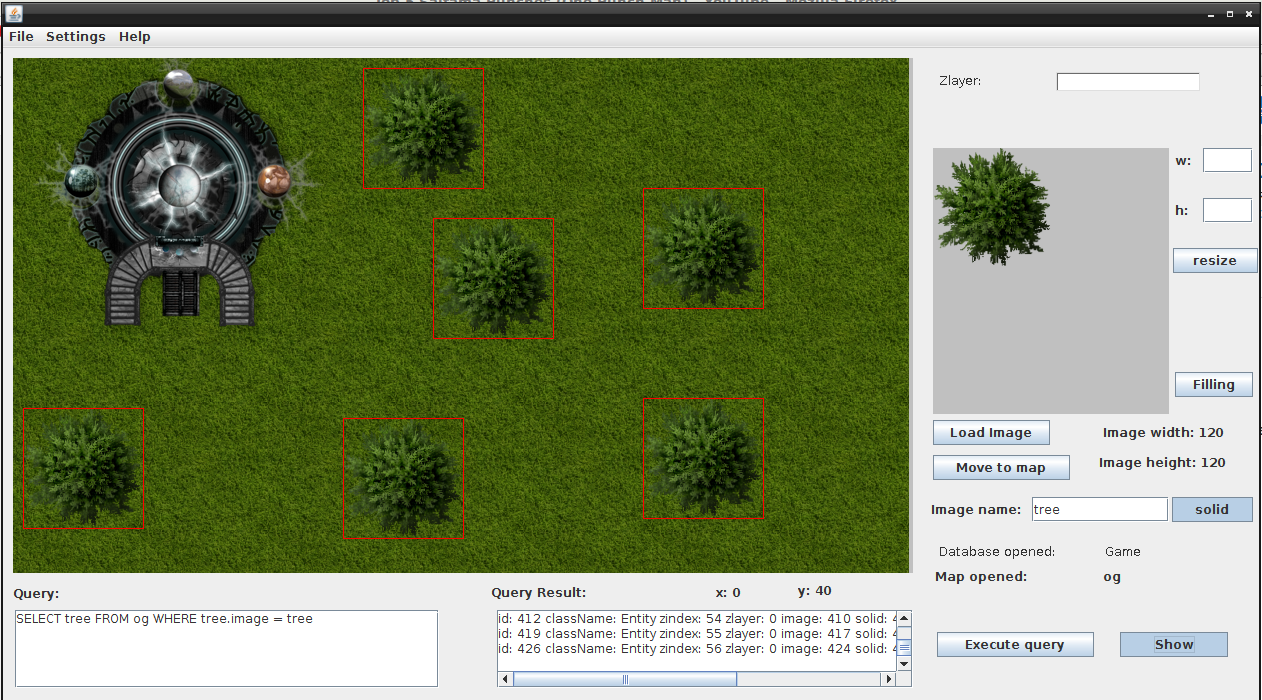
\includegraphics[scale=0.34]{images/editor}
		\caption{A Tile Editor használat közben}
		\label{fig:editor}
	\end{center}
\end{figure}

A \textit{File} menü alatt hozható létre új adatbázis, azon belül új térkép, illetve létező adatbázis, és térkép is innen érhető el. Ez a menüpont tartalmaz még egy \textit{Save} opciót is, ami arra szolgál, hogy a változtatásokat mentsük egy JSON fájlba. Ha módosítunk az adatbázison, de a \textit{Save} menüt nem használjuk, akkor az editor kikapcsolása után a memóriából az összes változtatás eltűnik, az adatok perzisztens tárolásáról nem gondoskodik.

A \textit{Settings} menü egyetlen funkciót tartalmaz, a \textit{Camera Settings} beállítást, ami arra szolgál, hogy az irányító gombokkal (fel, le, jobbra, balra) mennyi pixelt ugorjon a kamera. Az alapértelmezett beállítás az, hogy az $y$ tengely és az $x$ tengely irányába is 10 pixellel mozduljon el.
Ez azért fontos, mert nem lehet egérrel képeket beszúrni, hanem a \textit{"Move to Map"} gombra kattintva szúr be egy képet a térképből látható terület bal felső sarkához igazítva. 
A \textit{"Filling"} gomb mögött implementáltam azt a funkciót, amely lehetővé teszi azt, hogy a beszúrandó képeket ne egyesével, hanem egy bizonyos területet kitöltve szúrhassunk be. Ez is egy kényelmi eszköz, mellyel megadhatunk egy befoglaló téglalapot, amelyet kitölt.

A \textit{Help} menü alatt található egy rövid használati útmutató az alkalmazáshoz.

A főablak legnagyobb részét a térkép teszi ki, ahová beilleszthetünk képeket. Mellette a \textit{zlayer} szövegdoboz arra szolgál, hogy egy számot írjunk bele, aminek akkor van jelentősége, amikor egy képet szúrunk a térképre. Ez a háttérben lefutó \textit{INSERT} lekérdezésben a \texttt{LAYER} kulcsszó után szereplő attribútum. Ha ezt a mezőt nem töltjük ki, akkor sincs semmi probléma, olyankor a lekérdezés automatikusan 0 értéket vesz fel a \textit{zlayer}-nek.

A nagy térkép mellett látható egy kisebb téglalap is, amelyben képek jelenhetnek meg. Ennek az a funkciója, hogy a beszúrandó képeket megnézhetjük ott, illetve a mellette lévő két szövegdobozban (w, h) átméretezhetjük azt. 

A \textit{"LoadImage"} gomb segítségével érhetjük el a fájlrendszert, és tölthetünk be onnan képet az imént említett dobozba.

Az \textit{ImageWidth} és \textit{ImageHeight} feliratok az aktuálisan betöltött kép attribútumai, ez az információ hasznos lehet, mert így a kamerát beállíthatjuk, hogy milyen mértékben mozduljon el felhasználói beavatkozásra, és a betöltött képet kényelmesebben szúrhatjuk be.

Ha a \textit{"Move to Map"} gombra kattintunk, viszont az \textit{Image Name} szövegdobozba nem adtuk meg a beszúrandó kép nevét, akkor az alkalmazás figyelmeztetni fog, hogy ezt tegyük meg. Amit abba a szövegdobozba írunk, az a beszúrandó \texttt{Entity} objektum image attribútumának lesz az értéke. 

A \textit{"solid"} az egy \texttt{JToggleButton}, ami azt jelenti, hogy két állapota van, vagy lenyomva van, vagy alapértelmezetten. Ha nincs aktiválva, akkor a beszúrandó új \texttt{Entity} objektum \texttt{solid} attribútumának értéke \texttt{false} lesz, ha aktiválva van akkor \texttt{true}. Ez azért fontos mert az ütközésvizsgálat ezen attribútumra épül, ugyanis ha egy entitás nem \textit{solid}, akkor az ütközésvizsgálat szempontjából semleges.

Az \textit{Image Name} szövegdoboz alatt két felirat látható, amelyek az épp aktuálisan megnyitott adatbázis és map nevét mutatják. Ha megnyitjuk az editort akkor ezek értelemszerűen még nem tartalmaznak értéket, ezért ilyenkor a "-" karakter látható feltüntetve.

Az \textit{"Execute Query"} gombra kattintva a \textit{Query} Szövegmezőben látható lekérdezés fog lefutni, aminek eredménye a \textit{Query Result} szövegmezőben látható. Ha bekapcsolja a felhasználó a \textit{debug} módot, akkor e térképen a lekérdezés eredményei láthatóvá válnak oly módon, hogy egy piros taglalap rajzolódik köré. A \textit{debug} módot a \textit{show} \texttt{JToggleButton} aktiválásával lehet bekapcsolni. 

